\documentclass[main.tex]{subfiles}

\begin{document}
\KOMAoptions{twoside=false}
\begin{fullsizetitle}
	\hspace{2cm}
	
\includegraphics[width=5cm, valign=c]{images/logos/up-uhh-logo-u-2010-u-farbe-u-cmyk}
	\hspace{1cm}
	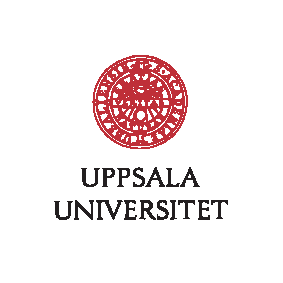
\includegraphics[width=4cm, valign=c]{images/logos/UU_logo_CMYK}\par
	\vspace{1\baselineskip}
	\hspace{0.1\textwidth}
	\smash{\textcolor{UHHgray}{\rule[-21.9cm]{1pt}{0.75\textheight}}}\hspace{10pt}
    \begin{minipage}[t][0.75\textheight][t]{0.8\textwidth}
    \begin{FlushLeft}
        {\Large \textsf{\textcolor{UHHgray}{Master thesis}}\par}

        {\huge \textsf{\textcolor{black}{Superconducting Phase Stiffness and Coherence Length From a Finite Momentum Pairing Constraint}}\par}

       \vspace{1\baselineskip}
       
       \textsf{\textcolor{UHHgray}{Hamburg, April 2025}}
    \end{FlushLeft}

    \vfill
    
    \begin{FlushLeft}
    	Tjark Sievers (7147558)\par
        Department of Physics\par
        First reviewer: Prof.\,Dr.\,Tim Wehling\par
        Second reviewer: Prof.\,Dr.\,Annica Black-Schaffer (Uppsala University)\par
    \end{FlushLeft}
    \end{minipage}
\end{fullsizetitle}



\thispagestyle{plain}

\epigraph{Even Einstein [...] had attempted to construct a theory of superconductivity. Fortunately, I was unaware of these many unsuccessful attempts. So when John invited me to join him (he, somehow, neglected to mention these previous efforts), I decided to take the plunge.}{Leon Cooper \par \enquote{Remembrance of Superconductivity Past}, BCS: 50 Years \cite{cooperBCS50Years2010}.}

\vspace*\fill

\bigskip

\noindent
Typeset with {\LaTeX} in TeX Gyre Pagella, \textsf{TeX Gyre Heros}, and \texttt{TeX Gyre Cursor}.

\end{document}
